\documentclass[12pt]{article}

\usepackage{sbc-template}

\usepackage{graphicx,url}

\usepackage[brazil]{babel}   
%\usepackage[latin1]{inputenc}  
% UTF-8 encoding is recommended by ShareLaTex
\usepackage[utf8]{inputenc}
\usepackage{listings}

\widowpenalty=10000


\clubpenalty=10000

\usepackage{color}
\usepackage{float}

\definecolor{codegreen}{rgb}{0,0.6,0}
\definecolor{codegray}{rgb}{0.5,0.5,0.5}
\definecolor{codepurple}{rgb}{0.58,0,0.82}
\definecolor{backcolour}{rgb}{0.95,0.95,0.92}
 
\lstdefinestyle{mystyle}{
    backgroundcolor=\color{backcolour},   
    commentstyle=\color{codegreen},
    keywordstyle=\color{magenta},
    numberstyle=\tiny\color{codegray},
    stringstyle=\color{codepurple},
    basicstyle=\footnotesize,
    breakatwhitespace=false,         
    breaklines=true,                 
    captionpos=b,                    
    keepspaces=true,                 
    numbers=left,                    
    numbersep=5pt,                  
    showspaces=false,                
    showstringspaces=false,
    showtabs=false,                  
    tabsize=2
}
 
\lstset{style=mystyle}
\renewcommand{\lstlistingname}{Quadro}

\sloppy

\title{Aceleração de uma Aplicação Científica com OpenCL: Regularização de Dados Sísmicos}

\author{Vanderson Martins do Rosario\inst{1}}


\address{Instituto de Computação -- Universidade Estadual de Campinas (Unicamp)\\
  Campinas -- SP -- Brasil
}

\begin{document} 

\maketitle
     
\begin{resumo} 
Este trabalho apresenta uma sequência de transformações aplicadas sobre um código, inicialmente sequêncial, para que esse obtenha o máximo desempenho sobre um processador \textit{multicore} e uma placa de vídeo por meio do \textit{framework} OpenCL. Durante o desenvolvimento do trabalho, diversos experimentos foram realizados para medir a eficiência de cada implementação e de cada transformação, tanto para guiá-las quanto para mostrar os impactos das mesmas. Nessa seção, apresentamos a lista dos materias utilizados e as técnicas utilizadas para realização e medição dos experimentos.
\end{resumo}


\section{Introdução}
Este trabalho apresenta uma sequência de transformações aplicadas sobre um código, inicialmente sequêncial, para que esse obtenha o máximo desempenho sobre um processador \textit{multicore} e uma placa de vídeo por meio do \textit{framework} OpenCL. Durante o desenvolvimento do trabalho, diversos experimentos foram realizados para medir a eficiência de cada implementação e de cada transformação, tanto para guiá-las quanto para mostrar os impactos das mesmas. Nessa seção, apresentamos a lista dos materias utilizados e as técnicas utilizadas para realização e medição dos experimentos.

Este trabalho apresenta uma sequência de transformações aplicadas sobre um código, inicialmente sequêncial, para que esse obtenha o máximo desempenho sobre um processador \textit{multicore} e uma placa de vídeo por meio do \textit{framework} OpenCL. Durante o desenvolvimento do trabalho, diversos experimentos foram realizados para medir a eficiência de cada implementação e de cada transformação, tanto para guiá-las quanto para mostrar os impactos das mesmas. Nessa seção, apresentamos a lista dos materias utilizados e as técnicas utilizadas para realização e medição dos experimentos.

Este trabalho apresenta uma sequência de transformações aplicadas sobre um código, inicialmente sequêncial, para que esse obtenha o máximo desempenho sobre um processador \textit{multicore} e uma placa de vídeo por meio do \textit{framework} OpenCL. Durante o desenvolvimento do trabalho, diversos experimentos foram realizados para medir a eficiência de cada implementação e de cada transformação, tanto para guiá-las quanto para mostrar os impactos das mesmas. Nessa seção, apresentamos a lista dos materias utilizados e as técnicas utilizadas para realização e medição dos experimentos.

Este trabalho apresenta uma sequência de transformações aplicadas sobre um código, inicialmente sequêncial, para que esse obtenha o máximo desempenho sobre um processador \textit{multicore} e uma placa de vídeo por meio do \textit{framework} OpenCL. Durante o desenvolvimento do trabalho, diversos experimentos foram realizados para medir a eficiência de cada implementação e de cada transformação, tanto para guiá-las quanto para mostrar os impactos das mesmas. Nessa seção, apresentamos a lista dos materias utilizados e as técnicas utilizadas para realização e medição dos experimentos.
\section{Materiais e Métodos}

Este trabalho apresenta uma sequência de transformações aplicadas sobre um código, inicialmente sequêncial, para que esse obtenha o máximo desempenho sobre um processador \textit{multicore} e uma placa de vídeo por meio do \textit{framework} OpenCL.

Durante o desenvolvimento do trabalho, diversos experimentos foram realizados para medir a eficiência de cada implementação e de cada transformação, tanto para guiá-las quanto para mostrar os impactos das mesmas. Nessa seção, apresentamos a lista dos materias utilizados e as técnicas utilizadas para realização e medição dos experimentos.

\subsection{Materiais}

Todos os experimentos foram realizados sobre uma mesma máquina, Dell Optiplex 9020, equipado com um processador Intel(R) Core(TM) i5-4590 CPU @ 3.30GHz com quatro unidades de processamento e uma GPU Intel(R) HD Graphics 4600 com 20 unidades de processamento com frequência máxima de 1150 MHz. Ainda, a máquina é equipada com 2 pentes de 4GB DDR3 SDRAM de 1600MHz em multiplos canais.

% Precisa da versão do CENTOS 
%TODO
Para compilar o código fonte, foi utilizado o GCC versão 4.8.5 sobre a plataforma CentOS com um \textit{third-party kernel}: 4.4.13\-1.el7.elrepo.x86\_64. Entre os frameworks utilizados, o OpenMP na versão 3.1 e o OpenCL 1.2 com o driver da Intel na versão 16.4.4.47109.

Para todos os experimentos, o código fonte foi compilado com o comando apresentado no Quadro \ref{comandogcc}.\\
\begin{lstlisting}[language=bash, caption=Comando para compilar o código fonte dos experimentos., label=comandogcc]
$ gcc -O3 --std=c99 reg.c semblance.c su.c -lm -I. -lOpenCL -fopenmp
\end{lstlisting}

%As variáveis de ambiente do sistema .... %TODO


\subsection{Experimentos  e Código Fonte}

Utilizou-se, para obter-se as métricas de execução de todos os experimentos, a ferramenta Perf do Linux com o comando do Quadro \ref{comandoperf}. Para cada experimento, foram repetidas 20 execuções seguidas e feito a média dos valores obtidos, levando-se em consideração a lei dos grandes números. Dessa forma, para todos os gráficos apresentados nesse trabalho é mostrado os valores da média juntamente com o desvio padrão. \\ %TODO citar lei dos grandes números.

\begin{lstlisting}[language=bash, caption=Comando para mensurar as métricas de execução., label=comandoperf]
$ perf stat -B -e cache-references,cache-misses,cycles,instructions,branches,branch-misses,faults,migrations
\end{lstlisting}

Ainda, em todos os gráficos de tempo de execução do trabalho, os tempos de execução são mostrados dividos em duas partes: (1) tempo de inicialização e (2) tempo de execução. Onde, o (1) tempo de inicialização é o tempo necessário para inicialização e configuração do OpenCL, alocação da memória, leitura do código-fonte do \textit{kernel}, leitura do arquivo com os dados de entrada e compilação do \textit{kernel}; e o (2) tempo de execução é o tempo para execução do \textit{kernel} mais o tempo para transferência dos dados de entrada e saída. Para medir esses dois tempos, o código foi instrumentado com a função do Quadro \ref{functime}. \\

\begin{lstlisting}[language=c, caption=Função utilizada para calcular o tempo de execução de trexos de código, label=functime]
#include <sys/time.h>

double mysecond() {
  struct timeval tp;
  gettimeofday(&tp ,NULL);
  return ((double) tp.tv_sec + (double) tp.tv_usec * 1.e-6);
}
\end{lstlisting}

O código fonte apresentado e citado no trabalho pode ser obtido por meio do repositório git hospedado no github.com (\url{https://github.com/vandersonmr/REG}). Todas as etapas apresentadas na Seção \ref{desenvolvimento} podem ser vistas pelo histório de \textit{commits} do repositório. Por exemplo, o código com as transformações citadas na Seção \label{desenvolvimento} pode ser obtido com os comandos git do Quadro \ref{comandogit}. \\

\begin{lstlisting}[language=bash, caption=Comando para navegar pelas transformações apresentadas no artigo., label=comandogit]
$ git clone https://github.com/vandersonmr/REG
$ git log --oneline
$ git reset --hard HashAqui
\end{lstlisting}

\section{Desenvolvimento e Resultados} \label{desenvolvimento}

Dado uma implementação sem muitas otimizações de uma solução sequêncial para a regularização de dados sísmicos\ref{borin}, foram primeiramente testados o desempenho dessa solução per si, em seguida o de uma simples paralelização dessa solução com OpenMP e com a paralelização com OpenCL depois de aplicado um conjunto de otimizações.

Nessa seção, apresentamos uma breve análise do código original, sequêncial (\ref{seq}); da paralelização com OpenMP (\ref{omp}), da paralelização com OpenCL (\ref{ocl}), seguido da explicação das diversas otimizações aplicadas sobre a última e seus impactos no desempenho da mesma.

\subsection{Código Sequêncial} \label{seq}

A implementação sequêncial pode ser dividido em três grandes partes, a saber: 

\begin{itemize}
\item \textbf{Inicialização}: Nessa parte, toda contida no arquivo reg.c, o programa lê os parametros passados para o executável (\ref{param}), lê um arquivo contendo os dados sísmicos (\ref{file}) e em seguida cria e preenche estruturas de dados que seram usados pelo \textit{kernel} (\ref{struct}). 

\begin{lstlisting}[language=c, caption=Leitura dos parametros passados para o executável., label=param]
    float m0 = atof(argv[1]);
    float h0 = atof(argv[2]);
    float t0 = atof(argv[3]);
    float tau = strtof(argv[4], NULL);
    
    float p0[5], p1[5];
    int np[5];
 
    for (i = 0; i < 5; i++) {
        p0[i] = atof(argv[5 + 3*i]);
        p1[i] = atof(argv[5 + 3*i + 1]);
        np[i] = atoi(argv[5 + 3*i + 2]);
    }
\end{lstlisting}

Para cada experimento, foram testados 3 conjuntos de parametros como entrada, a saber:

\begin{itemize}
\item Param1: 
\begin{lstlisting}[language=bash]
"4120 -480 1.124 0.005
-0.1     0.1     20 
-0.00143 0.00057 20 
 7.8e-07 9.8e-07 20 
-1.0e-07 1.0e-07 20 
-1.0e-07 1.0e-07 20"
\end{lstlisting}
\item Param2:
\begin{lstlisting}[language=bash]
"4120 -480 1.94 0.005
-0.00088484  0.00111516 20 
-0.001194    0.000806   20 
 6.4e-07     8.4e-07    20 
 6.0e-10     8.0e-10    20 
 4.61e-08    6.61e-08   20"
\end{lstlisting}
\item Param3:
\begin{lstlisting}[language=bash]
"4120 -480 2.255 0.005
-0.001147   0.000853  20 
-0.001139   0.000861  20 
 4.396e-07  5.396e-07 20 
 3.002e-07  4.102e-07 20 
-2.101e-07  0.101e-07 20"
\end{lstlisting}
\end{itemize}

\begin{lstlisting}[language=c, caption=Leitura do arquivo com os dados sismícos., label=file]
    char *path = argv[20];
    FILE *fp = fopen(path, "r");
	...
    su_trace_t tr;
    vector_t(su_trace_t) traces;
    vector_init(traces);

    while (su_fgettr(fp, &tr)) {
        vector_push(traces, tr);
    }
\end{lstlisting}

\begin{lstlisting}[language=c, caption=Preenchimento da estrtura de dados., label=struct]
   aperture_t ap;
    ap.ap_m = 0;
    ap.ap_h = 0;
    ap.ap_t = tau;
    vector_init(ap.traces);
    for (int i = 0; i < traces.len; i++)
        vector_push(ap.traces, &vector_get(traces, i));
\end{lstlisting}


A inicialização ocupa pouco tempo na execução total do programa. A leitura do arquivo é a parte mais demorada (\ref{file}), principalmente quando o programa é executado pela primeira vez. Se executado em sequência, o arquivo já está em \textit{cache} e o tempo da etapa de inicialização cai drasticamente.
\\
\item \textit{\textbf{Kernel}}: Nessa parte, contida no arquivo reg.c e semblance.c, a função \textit{compute\_max} (\ref{max}) chama a função \textit{semblance\_2d} (kernel) diversas vezes. A função \textit{semblance\_2d} (\ref{semblance}), medido pelo Perf, ocupa 97\% do tempo de exeução do programa, portanto, é o trexo mais quente e mais interessante para ser otimizado. 

\begin{lstlisting}[language=c, caption=Corpo da função \textit{compute\_max}., label=max]
for (int ia = 0; ia < np[0]; ia++) {
 float a = n0[0] + ((float)ia / (float)np[0])*(n1[0]-n0[0]);
 for (int ib = 0; ib < np[1]; ib++) {
   float b = n0[1] + ((float)ib / (float)np[1])*(n1[1]-n0[1]);
   for (int ic = 0; ic < np[2]; ic++) {
     float c = n0[2] + ((float)ic / (float)np[2])*(n1[2]-n0[2]);
     for (int id = 0; id < np[3]; id++) {
       float d = n0[3]+((float)id / (float)np[3])*(n1[3]-n0[3]);
       for (int ie = 0; ie < np[4]; ie++) {
         float e = n0[4]+((float)ie/(float)np[4])*(n1[4]-n0[4]);
         float st;
                       
         float s = semblance_2d(ap,a,b,c,d,e,t0,m0,h0,&st);
	  ...
        }
      }
   }
 }
}
\end{lstlisting}

Nota-se que o kernel possui uma frequência alta de execução por estar sendo chamado diversas vezes dentro da função \textit{compute\_max}. Podemos ver a quantidade de \textit{loops} aninhados, sendo a chamada está no nível mais profundo.

\begin{lstlisting}[language=c, caption=Corpo da função \textit{semblance\_2d}., label=semblance]
    for (int i = 0; i < ap->traces.len; i++) {
        tr = vector_get(ap->traces, i);

        float mx, my, hx, hy;
        su_get_midpoint(tr, &mx, &my);
        su_get_halfoffset(tr, &hx, &hy);

        float t = time_2d(A, B, C, D, E, t0, m0, my, h0, hy);
        int it = (int)(t * idt);

        if (it - tau >= 0 && it + tau < tr->ns) {
            for (int j = 0; j < w; j++) {
                int k = it + j - tau;
                float v = interpol_linear(k, k+1,
                        tr->data[k], tr->data[k+1],
                        t*idt + j - tau);
                num[j] += v;
                den[j] += v*v;
                _stack += v;
            }
            M++;
        } else if (++skip == 2) {
            return 0;
        }
    }
\end{lstlisting}

A função \textit{semblance\_2d} possui dois acessos a dados na memória, o primeiro, na linha 2, acessa os \textit{traces} e o seguindo, dentro do \textit{loop}, acessa \textit{data}. Ambos os acessos são sequênciais, por isso, acredita-se que tenham boa localidade.
\\
\item \textbf{Finalização}: Na última parte, é necessário selecionar entre todos os semblances calculados, o melhor. Esse é o trexo mais rápido na execução do código.

\end{itemize}

Testamos o desempenho do código sequêncial com as otimização O0, O2 e O3 com vetorização, apesar do compilador (gcc-4.8.5) não ter conseguido vetorizar o código. O resultado do desempenho médio para cada sequência de otimização pode ser visto no gráfico da Fígura \ref{fgsequencial}. O melhor desempenho foi obtido com as otimizações O3, sendo 7.66 segundos para Param1; 31.59 segundos para Param2 e 31.62 segundos para o Param3.

\begin{figure}[H]
\centering
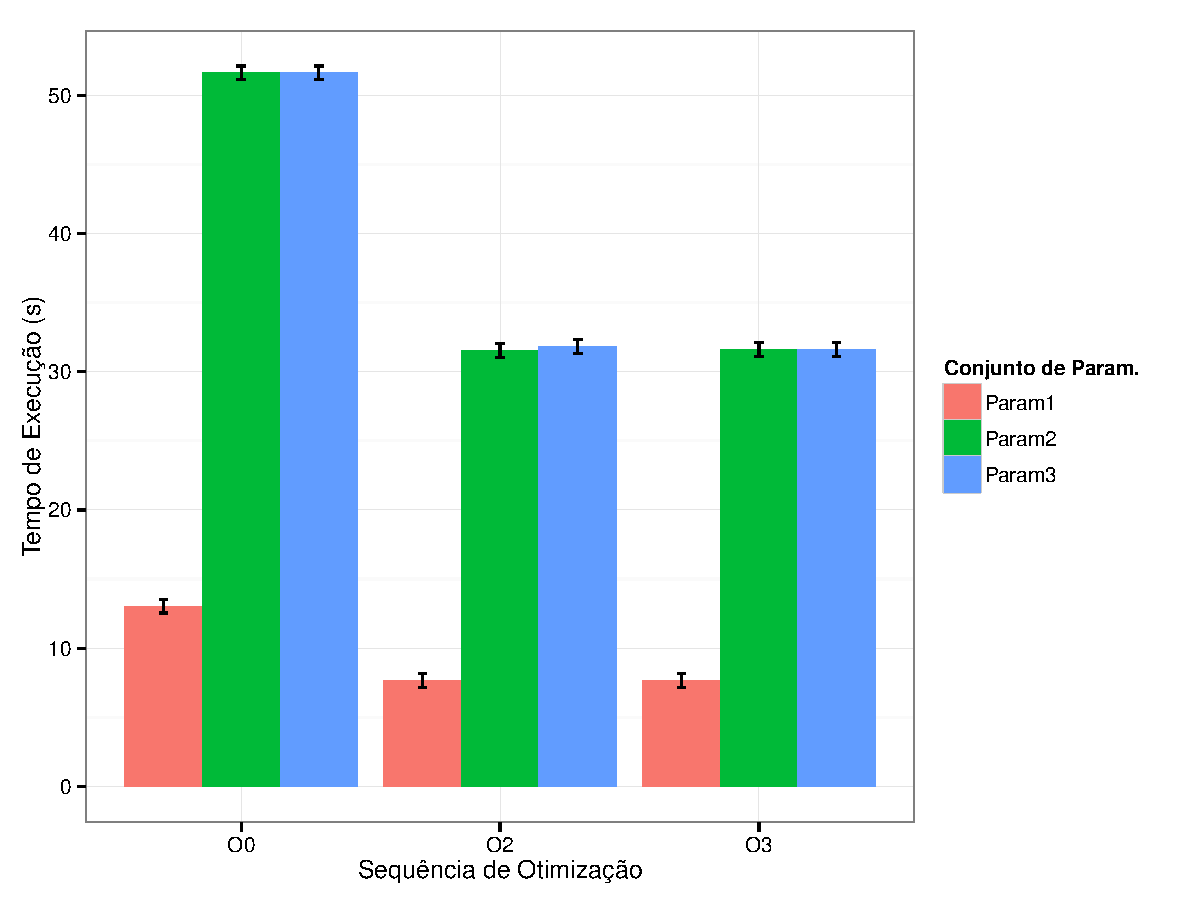
\includegraphics[width=0.8\textwidth]{seq.pdf}
\caption{Tempos de execução do código sequêncial compilado em O0, O2 e O3 para os três conjuntos de parametros de entrada.}
\label{fgsequencial}
\end{figure}

\subsection{Paralelização com OpenMP} \label{omp}

A paralelização utilizando-se do OpenMP foi feita de maneira bem simples: cada iteração do primeiro laço da função \textit{compute\_max} foi lançado em uma thread diferente pelo escalonador do OpenMP. Para isso, o \textit{pragma} do Quadro \ref{openmp} foi adiciona antes da linha do primeiro laço.
\\
\begin{lstlisting}[language=c, caption=\textit{Pragma} para paralelização com OpenMP., label=openmp]
    #pragma omp parallel for schedule(dynamic)
    for (int ia = 0; ia < np[0]; ia++) 
\end{lstlisting}

Além de adicionar o \textit{pragma}, como agora cada \textit{thread} calcula um \textit{semblance}, é preciso manter na memória o resultado de todas as \textit{threads} e depois iterar sobre eles para encontrar o melhor resultado. Com esse objetivo, o código do Quadro \ref{endomp} foi adicionado logo depois que a execução paralela do \textit{kernel} é finalizado. Note-se que foi adicionado diversos vetores que contém os resultados de cada \textit{thread}. \\

\begin{lstlisting}[language=c, caption=Código para selecionar o melhor resultado entre os resultados calculados por cada \textit{thread}., label=endomp]
    float ssmax = -1.0;
    *stack = 0;
    for (int ia = 0; ia < np[0]; ia++) {
        if (smax[ia] > ssmax) {
            *Aopt = _Aopt[ia];
            *Bopt = _Bopt[ia];
            *Copt = _Copt[ia];
            *Dopt = _Dopt[ia];
            *Eopt = _Eopt[ia];
            *stack = _stack[ia];
            *sem = smax[ia];
            ssmax = smax[ia];
        }
    }
\end{lstlisting}

Em seguida, notou-se que não havia a necessidade de utilizar a estrutura \textit{vector}, implementada no vector.h, no \textit{kernel}, porque, depois de lido o arquivo de entrada já se sabe a quantidade de traces. Portanto, foram feitas pequenas modificações no código para remover o uso do \textit{vector}. 

A Figura \ref{fgomp} mostra o resultado do tempo de execução da versão sequêncial (já apresentada) compilada com O3, da implementação com OpenMP e com o OpenMP sem o \textit{vector}. Como podemos ver pela figura, não se obteve melhorias no desempenho por não usar o \textit{vector}. Mas, a aplicação do OpenMP gerou um \textit{speedup} médio de $3.37x$, ou seja, para um processador com 4 unidades de processamento: 84\% de eficiência. Os desempenhos médios da implementação com OpenMP foram: 2.91 segundos para Param1; 8.43 segundos para Param2 e 8.44 segundos para Param3.

\begin{figure}[H]
\centering
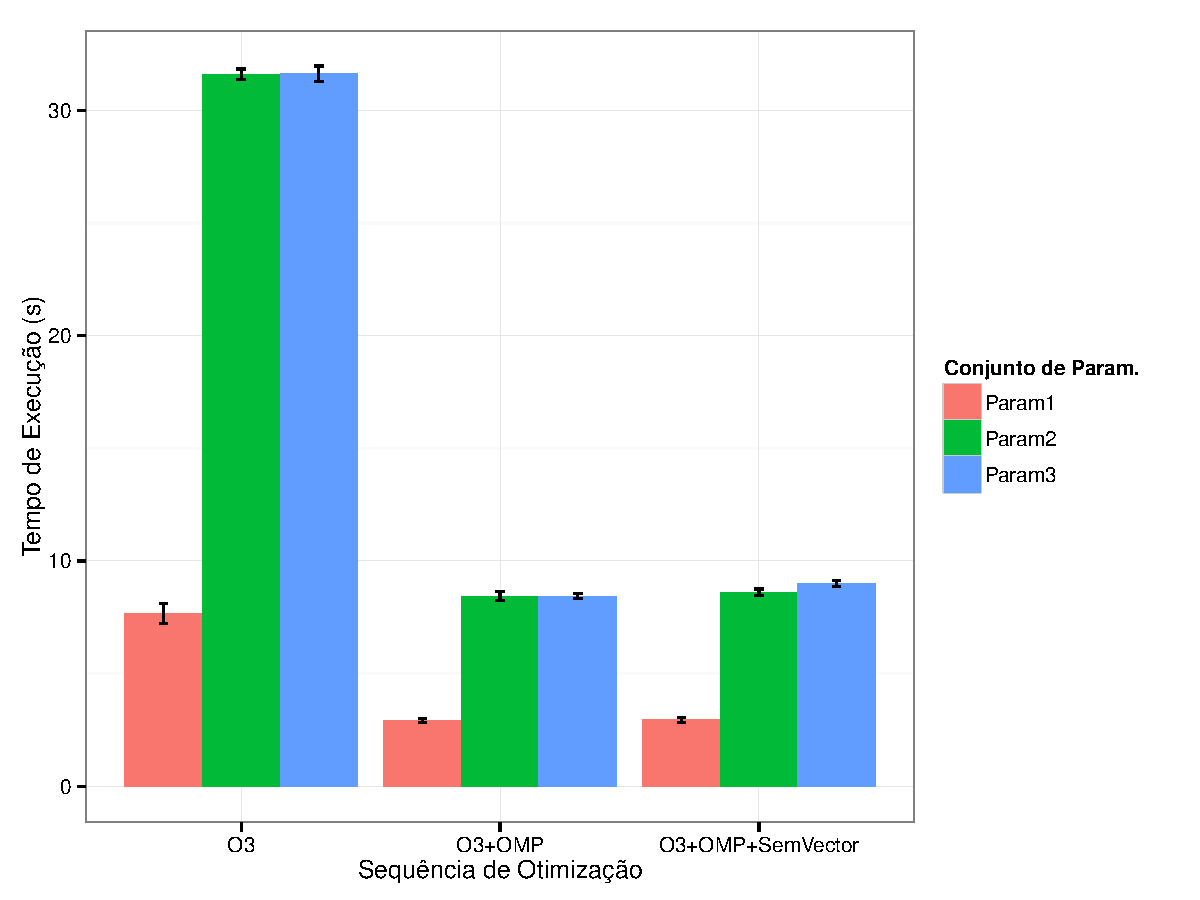
\includegraphics[width=0.8\textwidth]{omp.pdf}
\caption{Tempos de execução do código sequêncial compilado com O3, do código com OpenMP compilado em O3, e do código OpenMP compilado com O3 e sem a estrutura de vetores.}
\label{fgomp}
\end{figure}

O OpenCL permite que o código paralelizado seja executado em diversas arquiteturas, inclusive em GPUs. Isso não é possível com o OpenMP ou com o código original, portanto, as otimizações foram implementadas apenas para o OpenCL. Apesar disso, é possível perceber que a solução com OpenMP poderia se beneficiar das mesmas otimizações e, por isso, não é justo comparar o desempenho das duas implementações. Dessa forma, sabendo que o código OpenMP não pode ser executado nas mesmas plataformas e que não foram aplicadas as mesmas otimizações em sua implementação, o trabalho se concentra em obter o máximo desempenho sobre a implementação em OpenCL, sem se preocupar com comparações com a implementação com OpenMP.

A partir da próxima subseção, todos os resultados mostrados serão de experimentos compilados com O3.

\subsection{Paralelização com OpenCL} \label{ocl}

O OpenCL é um \textit{framework} para o desenvolvimento de programas que rodem em plataformas heterogênias consistindo de CPUs, GPUs, DSPs, FPGAs e outros processadores e aceleradores. O OpenCL especifica uma linguagem de programação baseada no C99 para programar esses dispositivos, provendo uma interface padrão para programação paralela \textit{task-based} e \textit{data-based}.

O primeiro objetivo desse trabalho é fazer com que a mesma forma de paralelização implementada em OpenMP seja portada para OpenCL para que possamos medir o desempenho na GPU e na CPU. 

Primeiro, foi necessário mover o código do \textit{kernel} e suas dependências nos arquivos semblance.h/c, su.h e reg.c para dentro de um único arquivo kernel.cl. Apesar de ser possível adicionar includes no kernel.cl, o código depois de incluido em único arquivo ficou pequeno o suficiente para não precisar ser separado.

Em seguida, foi preciso modificar a parte de inicialização para iniciar e configurar o OpenCL. Primeiro, declaramos as variáveis necessárias do \textit{framework} OpenCL, como podemos ver no quadro \ref{vars}.\\

\begin{lstlisting}[language=c, caption=Declaração das variáveis OpenCL., label=vars]
    cl_int          err;         //error code returned from calls
    size_t global;              //global domain size

    cl_device_id     device_id; //compute device id
    cl_context       context;   //compute context
    cl_command_queue commands;  //compute command queue
    cl_program       program;   //compute program
    cl_kernel        kernel;    //compute kernel
\end{lstlisting}

Durante a inicialização, também é necessário escolher qual dispositivo e qual plataforma será utilizado. O código do Quadro \ref{plat} seleciona a primeira GPU que for encontrada na primeira plataforma.\\

\begin{lstlisting}[language=c, caption=Selecionando a plataforma e o dispositivo OpenCL., label=plat]
    cl_uint numPlatforms;

    err = clGetPlatformIDs(0, NULL, &numPlatforms);
    if (numPlatforms == 0)
    {
        printf("Found 0 platforms!\n");
        return EXIT_FAILURE;
    }

    cl_platform_id Platform[numPlatforms];
    err = clGetPlatformIDs(numPlatforms, Platform, NULL);

    for (i = 0; i < numPlatforms; i++)
    {
        err = clGetDeviceIDs(Platform[i],  CL_DEVICE_TYPE_GPU, 1, &device_id, NULL);
        if (err == CL_SUCCESS)
        {
            break;
        }
    }
\end{lstlisting}

Assim que se tem uma plataforma e dispositivo definidos, cria-se um contexto e uma fila de execução para esse dispositivo. Nessa fila serão inseridos os kernels á serem executados. O código do Quadro \ref{context} mostra a criação do contexto, da fila e em seguida a leitura do arquivo "./kernel.cl".\\

\begin{lstlisting}[language=c, caption=Criação do contexto\, da fila de comandos e leitura do kernel.cl., label=context]
    context = clCreateContext(0, 1, &device_id, NULL, NULL, &err);

    commands = clCreateCommandQueue(context, device_id, 0, &err);

    FILE *kernel_fp;
    const char file_name[] = "./kernel.cl";
    kernel_fp = fopen(file_name, "r");
    size_t source_size;
    char *source_str;

    source_str = (char*) malloc(MAX_SOURCE_SIZE);
    source_size = fread(source_str, 1, MAX_SOURCE_SIZE, kernel_fp);
    fclose(kernel_fp);
\end{lstlisting}

A próxima etapa é compilar o código do kernel.cl. O trexo de código no Quadro \ref{compiling} mostra como compilar o código lido e como imprimir os logs gerados durante a compilação.\\

\begin{lstlisting}[language=c, caption=Compilando o kernel.cl., label=compiling]
    program = clCreateProgramWithSource(context, 1, (const char **)&source_str, (const size_t *)&source_size, &err);

    err = clBuildProgram(program, 1, &device_id, NULL, NULL, NULL);

    size_t log_size;
    err = clGetProgramBuildInfo(program, device_id, CL_PROGRAM_BUILD_LOG, 0, 
                                                              NULL, &log_size);
    char* build_log = (char* )malloc((log_size+1));
    err = clGetProgramBuildInfo(program, device_id, CL_PROGRAM_BUILD_LOG, 
                                                    log_size, build_log, NULL);
    build_log[log_size] = '\0';
    printf("\n--- Build log ---\n ");
    printf("%s\n\n", build_log);
    free(build_log);

    kernel = clCreateKernel(program, "compute_max", &err);
\end{lstlisting}

Por último é necessário copiar os dados que serão utilizados pelo \textit{kernel} para o dispositivo e adicionar o \textit{kernel} na fila de execução. Ainda, é preciso selecionar a dimensão do \textit{work size} e os tamanhos globais (espaço de iteração) e os tamanhos locais (tamanho dos \textit{work groups}). Essas etapas são feitas no código do Quadro \ref{initing}.\\ 

\begin{lstlisting}[language=c, caption=Copiando dados para o dispositivo e colocando \textit{kernel} na fila de execução., label=initing]
    cl_mem d_ps  = clCreateBuffer(context,
                           CL_MEM_READ_ONLY | CL_MEM_COPY_HOST_PTR,
                           sizeof(float)*5*2, ps, &err);
    checkError(err, "Creating buffer d_ps");
	...
    cl_mem d_data  = clCreateBuffer(context,
                           CL_MEM_READ_ONLY | CL_MEM_COPY_HOST_PTR,
                           sizeof(float)*ap.len*2052, data, &err);
    checkError(err, "creating buffer d_data");


    cl_mem d_results = clCreateBuffer(context, CL_MEM_READ_WRITE, 
				       sizeof(float)*7*np[0]*np[1]*np[2], NULL, &err);
    checkError(err, "Creating buffer d_results");

    err  = clSetKernelArg(kernel, 0, sizeof(d_ap), &d_ap);
    err |= clSetKernelArg(kernel, 1, sizeof(d_dm), &d_dm);
	...
    checkError(err, "Setting kernel arguments"); 
    
    size_t global_work_size[3] = {np[0], np[1], np[2]};
    size_t local_work_size[3] = {4, 4, 4};

    err = clEnqueueNDRangeKernel(commands, kernel, 3, NULL, global_work_size, 
                                                local_work_size, 0, NULL, NULL);
\end{lstlisting}

A inicialização com OpenCL tem um \textit{overhead} muito maior do que a do OpenMP. Os trexos de códigos descritos levam em torno de 100x mais tempo do que a inicialização do OpenMP. Por exemplo, nos últimos resultados com OpenCL, a inicialização chega, nos piores casos, a representar 42\% do tempo de execução.

Para uma primeira implementação, escolhemos 1 dimensão para o espaço de iteração, sendo que o espaço de iteração dessa dimensão é o primeiro laço como na implementação do OpenMP. Dessa forma, substituimos o laço do \textit{kernel} por um get\_global\_id(0). Assim, temos uma versão paralela com OpenCL que segue o mesmo princípio de paralelização que a implementação do OpenMP. As principais diferenças são: (1) o compilador do \textit{kernel} agora será o \textit{driver} da Intel; (2) o escalonador não mais será o do OpenMP, mas sim do \textit{Driver} da Intel; e (3), agora é preciso falar cópia de dados do \textit{host} para o dispositivo. 

A comparação do tempo de execução das duas implementações, OpenMP e OpenCL, pode ser visto no gráfico da Fígura \ref{fgcl}. Pode-se notar que o tempo de execução foi bastante próximo para as duas implementações, contudo o OpenCL obteve resultados piores do que o do OpenMP - provavelmente por causa do \textit{overhead} de inicialização, compilação e cópia dos dados.

Os resultados da Fígura \ref{fgcl} são na CPU, sendo que a implementação com OpenCL levou 3.35 segundos para o Param1, 9.078 para Param2 e 10.50 para o Param3. Não foi possível rodar o código na GPU, porque este tinha um desempenho deplorável e a execução foi abortada antes da finalização. Portanto, pode-se concluir que essa implementação da paralelização de apenas o primeiro laço não é uma boa solução para a GPU. 

\begin{figure}[H]
\centering
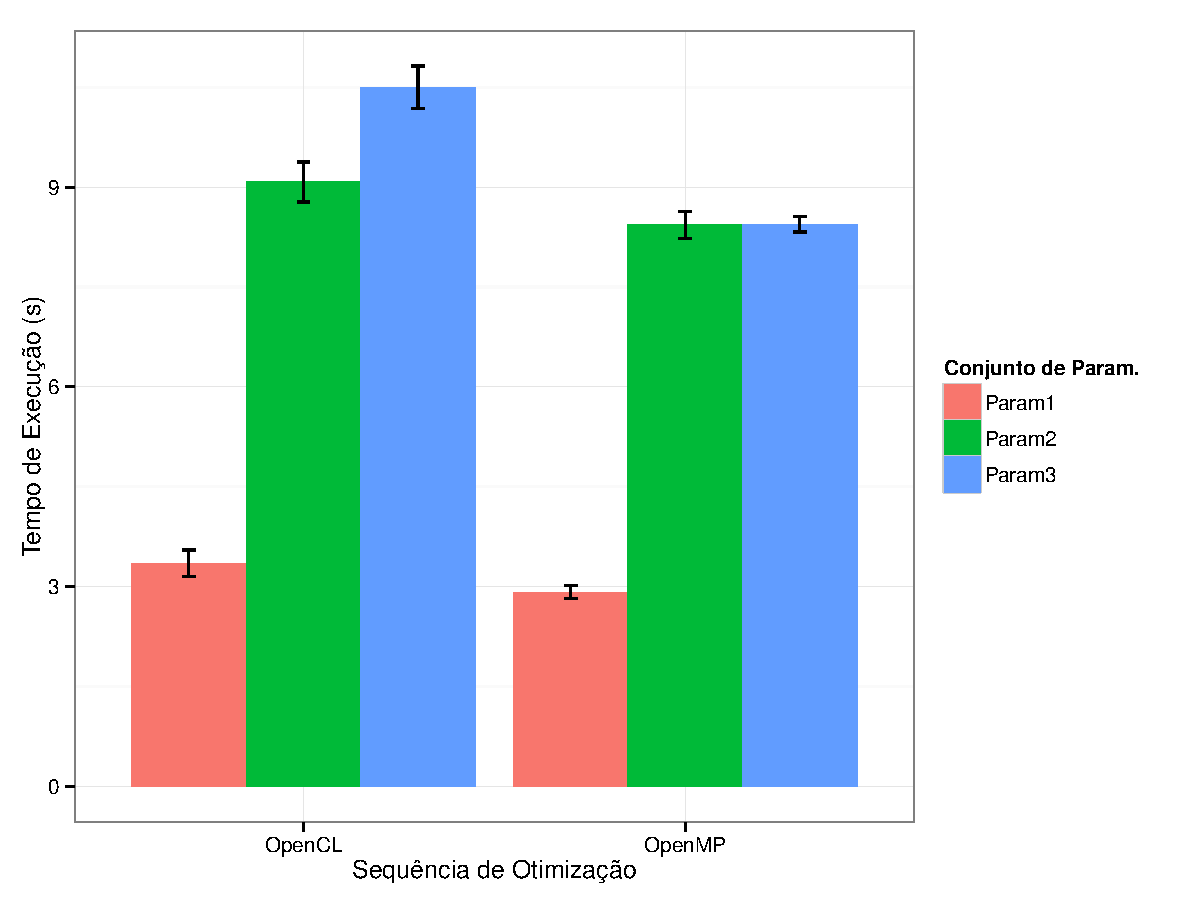
\includegraphics[width=0.8\textwidth]{ocl.pdf}
\caption{Tempos de execução do código com OpenMP e OpenCL sobre a CPU.}
\label{fgcl}
\end{figure}

Também foi possível notar, pelas estatísticas do Perf, que a quantidade de \textit{cache misses}, \textit{migrations} e \textit{branch-misses} para ambas as implementações se manteve estável.

\subsubsection{Removendo Dados Desnecessários}

A primeira transformação aplicada, foi retirar diversos dados que não estavam sendo utilizados pelo \textit{kernel}. No entanto, é importante manter duas estruturas, uma reduzia e outra original. Isso se da pelo fato que na leitura do arquivo de entrada, é feito um mapeamento dos blocos no arquivo a estrutura, ou seja, mudar a estrutura afetaria a leitura do arquivo. No entanto, uma vez lido, não há mais porque guardar esses dados ou transferi-los para os dispositivos OpenCL. No código do Quadro \ref{cstruct} podemos ver a estrutura depois de retirado as variáveis não utilizadas (su\_trace\_c). \\

\begin{lstlisting}[language=c, caption=Estrutura su\_trace depois de compactada., label=cstruct]
typedef struct su_trace_c su_trace_c_t;

struct su_trace_c {
	cl_short scalco; 
	cl_int sx; 
	cl_int sy; 
	cl_int gx; 
	cl_int gy; 
	cl_ushort ns; 
	cl_ushort dt; 
};
\end{lstlisting}


Esperava-se que essa redução tivesse um impacto significante no desempenho. Contudo, a diferença de desempenho não foi significante, 3.35 segundos para Param1, 8.94 para Param2 e 9.04 para Param3; como podemos ver no gráfigo da Fígura \ref{fgcstruct}. 

\begin{figure}[H]
\centering
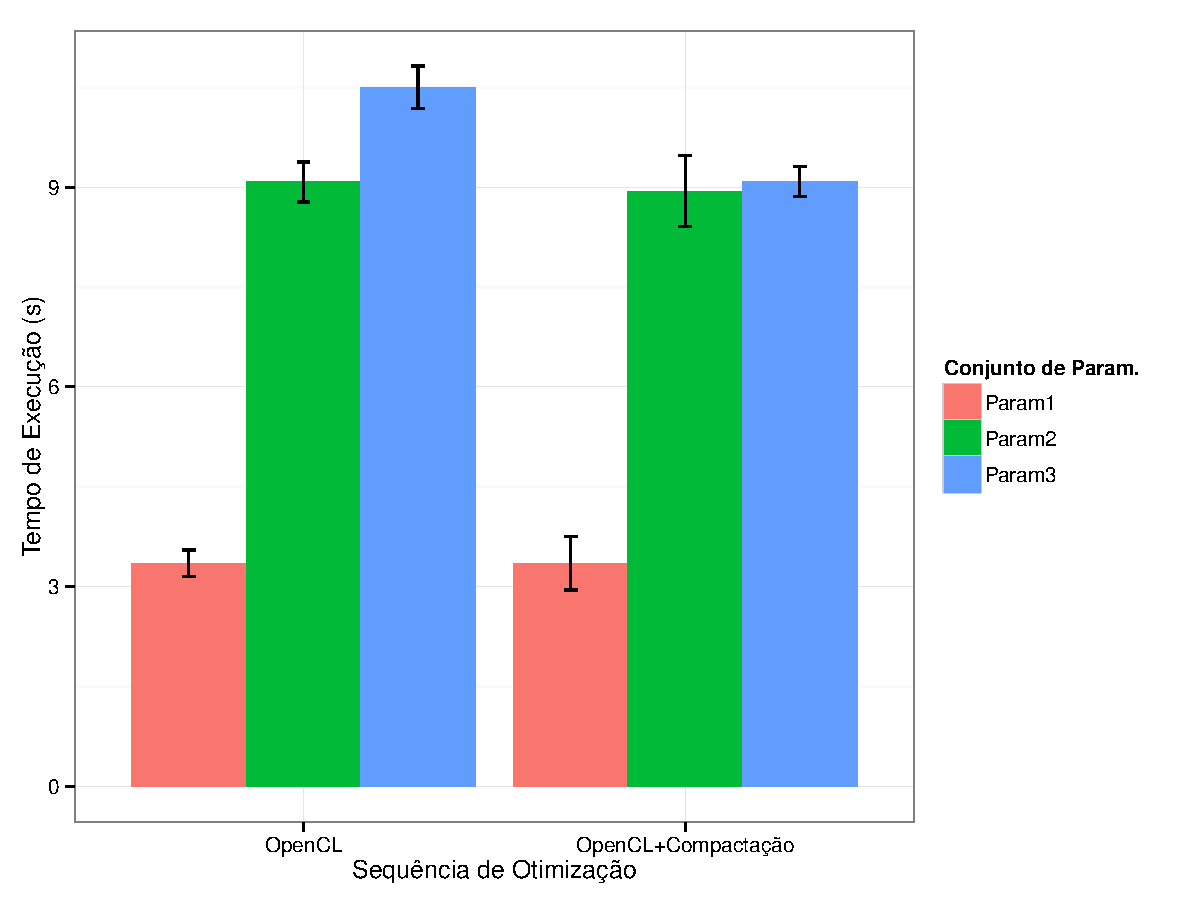
\includegraphics[width=0.8\textwidth]{oclcstruct.pdf}
\caption{Tempos de execução do código sem e com a remoção das variáveis não utilizadas.}
\label{fgcstruct}
\end{figure}
	

\subsubsection{Multidimensões} \label{multi} 

A segunda transformação aplicada com objetivo de melhorar o desempenho da implementação do código em OpenCL foi a de paralelizar não só o primeiro laço, mas os três primeiros. Dessa forma, temos um \textit{global work space} de 3 dimensões, onde cada dimensão tem o tamanho do tamnanhos das iterações dos laços.

Já o \textit{local work size} foi escolhido por meio das informações contidas no clinfo. Nele, é recomendado tamanhos para os \textit{work groups}. Testando diferentes valores multiplos dos valores recomendados pelo clinfo, chegamos nos \textit{local work size} de (4,4,4) para GPU e (2,2,2) para a CPU.

Com o aumento da quantidade de \textit{work itens} ocorre um aumento, também, de desempenho, já que possibilita que o escalonador mantenha uma maior utilização do \textit{hardware}. Não só obtivemos melhorias no desempenho com a CPU como também obtivemos, com 3 dimensões, o primeiro resultado aceitável com a GPU. Para mostrar esse efeito, testamos o desempenho com 2 laços paralelizados (2D) e com 3 laços paralelizados (3D). Os resultados podem ser visto no gráfico da Figura \ref{fgcl3d}. Sendo que o tempo de execução para a GPU foi de 1.02 segundos para Param1, 2.82 segundos para Param2 e 2.75 segundos para Param3. 

\begin{figure}[H]
\centering
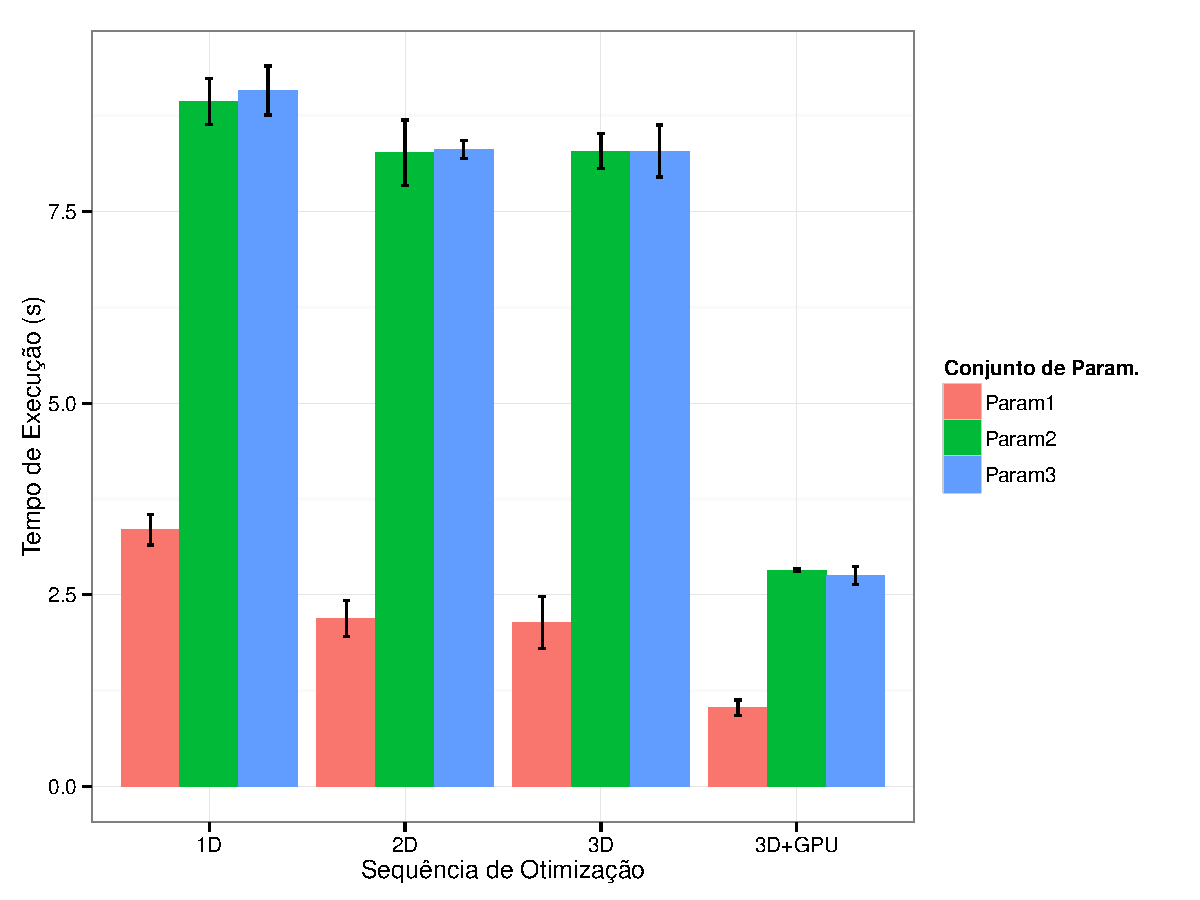
\includegraphics[width=0.8\textwidth]{ocl3d.pdf}
\caption{Tempos de execução do código com OpenCL sobre a CPU e GPU sobre multiplas dimensões.}
\label{fgcl3d}
\end{figure}

\subsubsection{\textit{Inlining} das Funções}

Apesar do manual da NVIDIA sobre OpenCL afirmar que o padrão do OpenCL é aplicar \textit{inlining} em todas as funções, existem diversos relatos em foruns especializados de relatos que o inlining manual trás melhorias no desempenho. Além disso, o \textit{inlining} manual permite que possam ser aplicados simplificações algébricas também manuais que o compilador pode não ser capaz de fazer. 

Após o \textit{inlining} manual de todas as funções chamadas pelo \textit{kernel}, obtivemos uma melhoria no desempenho que pode ser visto no gráfico da Figura \ref{fgcinline}. Sendo que o tempo de execução para a CPU foi de 1.48 segundos para Param1, 5.43 segundos para Param2 e 5.48 para Param3; e para a GPU foi de 0.75 segundos para Param1, 1.45 segundos para Param2 e 1.51 segundos para Param3.

\begin{figure}[H]
\centering
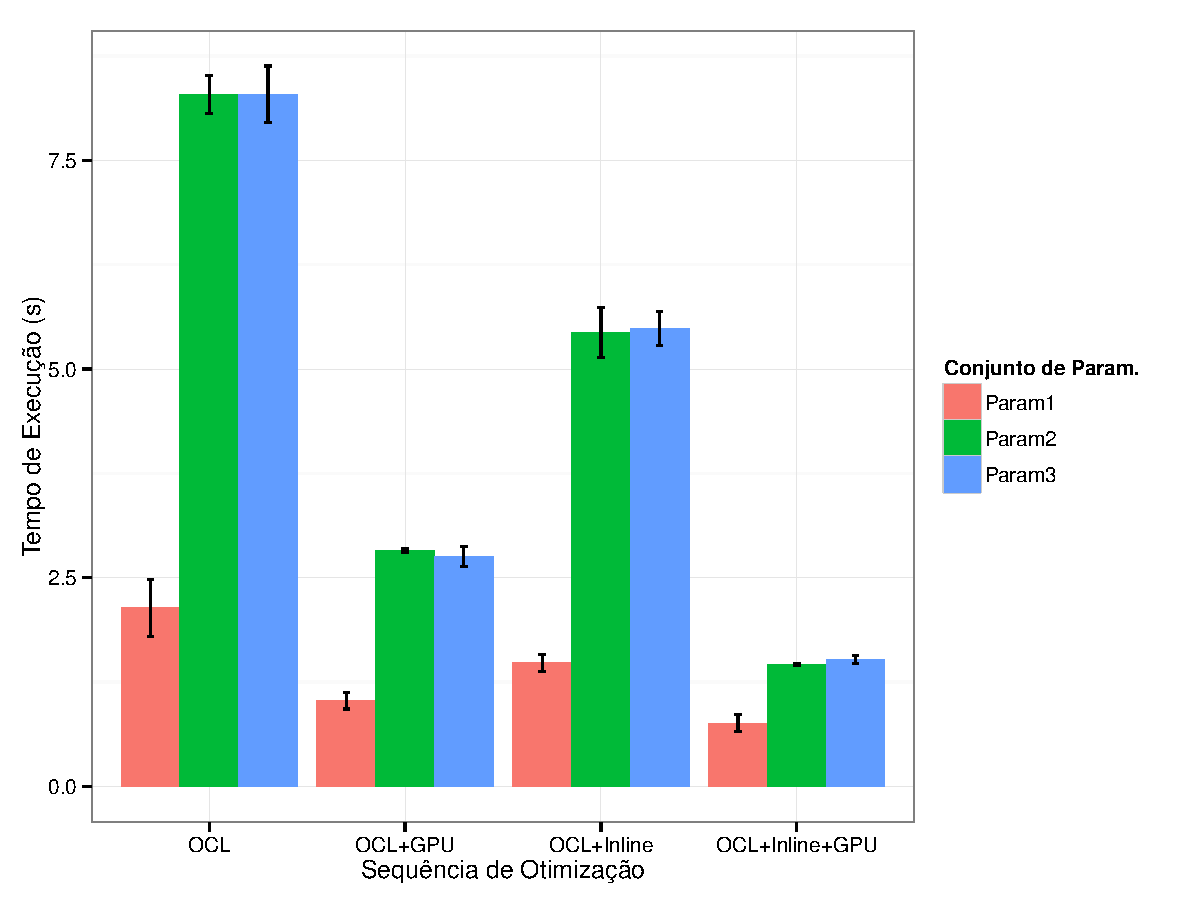
\includegraphics[width=0.8\textwidth]{oclinline.pdf}
\caption{Tempos de execução do código com OpenCL sobre a CPU e GPU antes e depois do \textit{inlining}.}
\label{fgcinline}
\end{figure}


\subsubsection{Simplificações Algébricas}

Após a aplicação do \textit{inlining} foi possível perceber diversas possibilidades de simplificação algébricas. Contudo, antes de aplicar as simplificações manualmente, testamos se ativar as simplificações que resultem em perda de precisão (-cl-mad-enable, -cl-unsafe-math-optimizations, -cl-fast-relaxed-math) iria resultar em melhoria do desempenho. Contudo, não ocorreu nenhuma melhoria de desempenho.

Portanto, resolvemos aplicar as transformações manualmente. Entretante, é importante lembrar que nesse momento, apesar de que nos resultados para as entradas testadas não houve mudança dos resultados, não podemos afirmar a corretude do programa. Dessa forma, assumimos que estamos fazendo um \textit{trade off} entre precisão e desempenho nessa etapa. 

O \textit{inlining} das funções time\_2d, su\_get\_midpoint e su\_get\_halfoffset não resultou em nenhuma otimizações. Contudo, o inlining da interpol\_linear, presente no trexo mais quente do \textit{kernel}, vista no Quadro \ref{interpol} , possibilitou diversas simplificações. \\

\begin{lstlisting}[language=c, caption=Trexo de chamada da função interpol\_linear antes do \textit{inlining}., label=interpol]
  float interpol_linear(float x0,float x1,float y0,float y1,float x)
  {
    return (y1 - y0) * (x - x0) / (x1 - x0) + y0;
  }
  ...
  if (it - tau >= 0 && it + tau < tr->ns) {
    for (int j = 0; j < w; j++) {
      int k = it + j - tau;
      float v = interpol_linear(k, k+1,
                                tr->data[k], tr->data[k+1],
                                t*idt + j - tau);
      num[j] += v;
      den[j] += v*v;
      _stack += v;
    }
    M++;
}
\end{lstlisting}

Trocando os valores de $(y1 - y0) * (x - x0) / (x1 - x0) + y0$ pelos valores da chamada da função, obtemos: 
$$(tr.data[k+1] - tr.data[k]) * (t*idt + j - tau - k) / (k + 1 - k) + tr.data[k+1] = $$
$$ = (tr.data[k+1] - tr.data[k]) * (t*idt + j - tau - k) + tr.data[k+1] \Rightarrow $$
Sabendo que $k = it + j - tau;$, temos:
$$ \Rightarrow (tr.data[k+1] - tr.data[k]) * (t*idt + j - tau - it - j + tau) + tr.data[k+1] = $$
$$ = (tr.data[k+1] - tr.data[k]) * (t*idt - it) + tr.data[k+1] \Rightarrow$$
Como $(t*idt - it)$ é independente da variável de indução, tiramos ele do laço:
$$ \Rightarrow (tr.data[k+1] - tr.data[k]) * v2 + tr.data[k+1] =$$
$$ = tr.data[k+1]*v2 - tr.data[k]*v2 + tr.data[k+1] = $$
$$ = tr.data[k+1]*v2 + tr.data[k]*(1-v2)$$.

O resultado pode ser visto no código do Quadro \ref{alg}.\\

\begin{lstlisting}[language=c, caption=Estrutura su\_trace depois de compactada., label=alg]
  int base = it - tau;
  if (base >= 0 && it + tau < 2502) {
    float v2 = (t*idt - it);
    for (int j = 0; j < w; j++) {
      int k = base + j;
      float v = tr->data[k+1]*v2 + tr->data[k]*(1-v2);
      num[j] += v;
      den[j] += v*v;
      _stack += v;
    }
    M++;
   }
\end{lstlisting}

Ainda, foi possível perceber que as chamadas das função su\_get\_midpoint, su\_get\_halfoffset e parte da função time\_2d no \textit{kernel} são independentes da variavel de indução do laço no qual estão inseridas. Portanto, optou-se por mover esse trexo do código para o host. Dessa forma, há, no host, um pré-calculo dos valores que seram utilizados posteriormente pelo \textit{kernel}.

Essas transformações resultaram em um impacto no desempenho na GPU, mas não tanto quanto na CPU, como podemos ver no gráfico da Fígura \ref{fgclsimpl}. Na CPU o desempenho foi de 1.075 segundos para Param1, 3.44 segundos para Param2 e 3.45 segundos para Param3.

\begin{figure}[H]
\centering
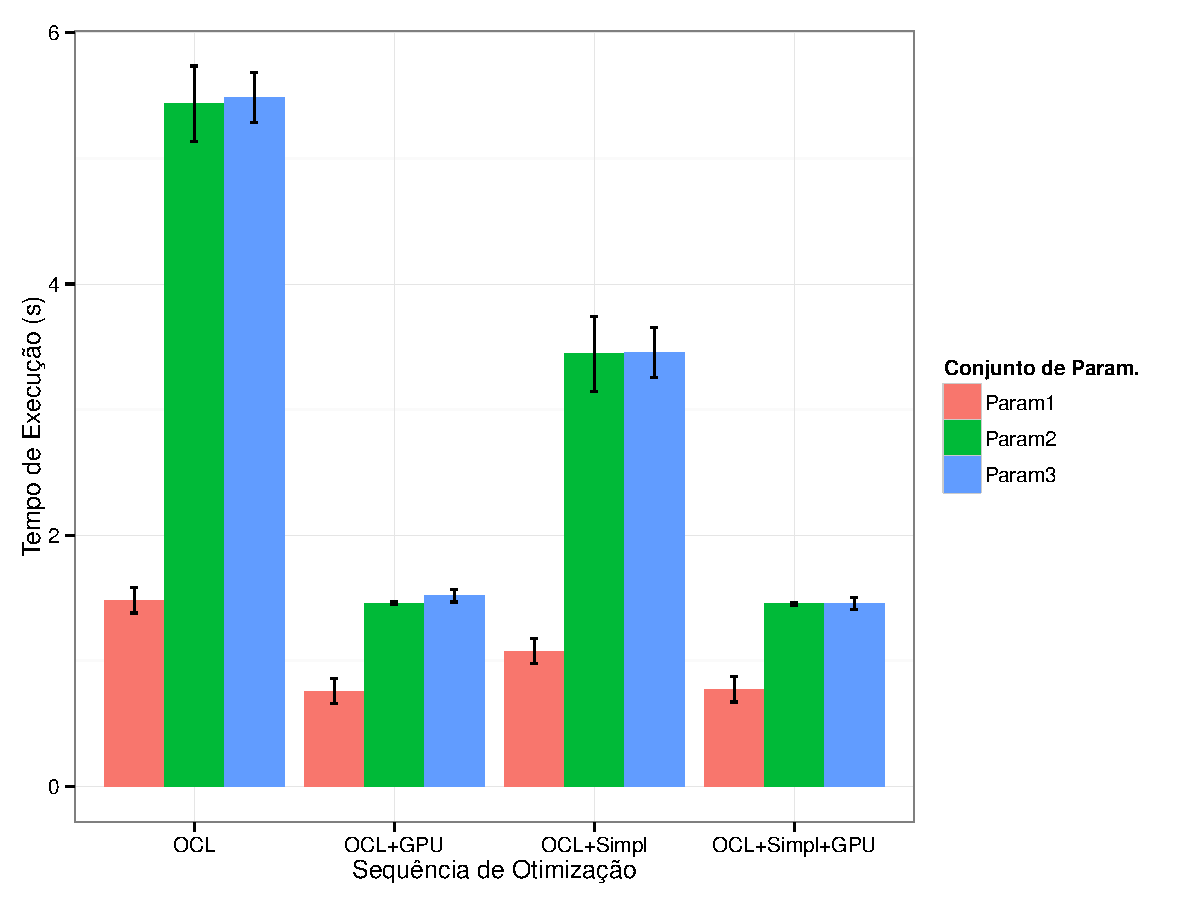
\includegraphics[width=0.8\textwidth]{oclsimpl.pdf}
\caption{Tempos de execução do código com OpenCL com \textit{inlining} sobre a CPU e GPU antes e depois das simplificações.}
\label{fgclsimpl}
\end{figure}

\subsubsection{\textit{Constant Memory Space}}

As GPUs possuem memórias constantes para texturas que são tão rápidas quanto a cache. Para aumentar o desempenho, movemos todas os dados que estavam na memória global, menos o "data", já que esse é grande de mais. Para isso, foi apenas necessário trocar as \textit{flags} \_\_global por \_\_constant na frente dos atríbutos do \textit{kernel}.

Essa modificação trouxe melhorias para o desempenho do código na GPU, mas não na CPU. O gráfico da Figura \ref{fgclconst} mostra o ganho de desempenho na GPU depois de aplicado a transformação.

\begin{figure}[H]
\centering
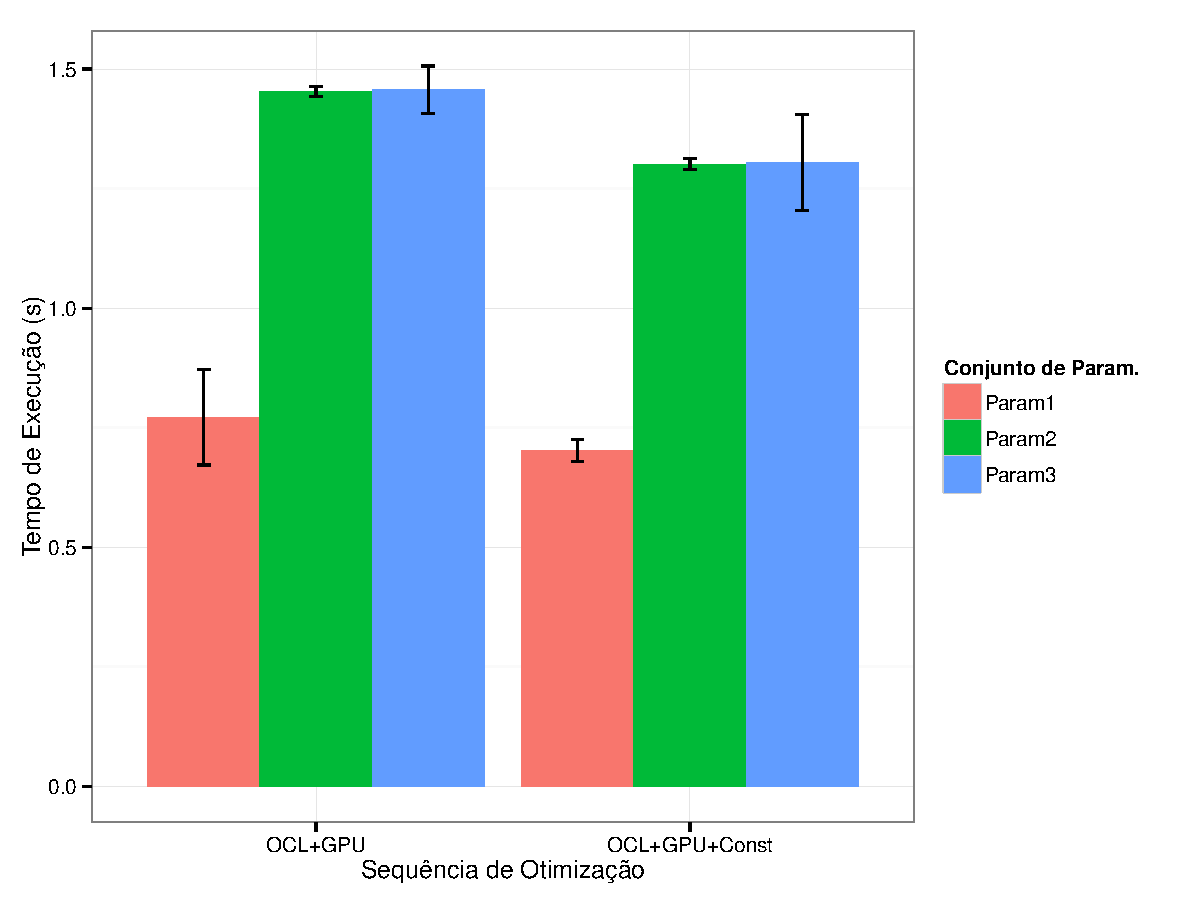
\includegraphics[width=0.8\textwidth]{oclconst.pdf}
\caption{Tempos de execução do código com OpenCL com \textit{inlining} sobre a GPU antes e depois de mover os dados para memória de constantes.}
\label{fgclconst}
\end{figure}

\subsubsection{Reduzindo a Pressão Sobre os Registradores }

Analisando o código e retirando trexos para verificar o impacto no desempenho, observou-se que o desempenho estava sendo limitado pela memória. Contudo, os dois acessos visíveis a memória estavam tendo bom aproveitamento da cache e quando retirados não afetavam em muito o desempenho. Em uma análise mais minuciosa, percebeu-se que o que estava gerando o gargalo no desempenho era a pressão sobre os registradores. Pela falta de registradores, a constante troca dos valores dos registradores para a memória estava delimitando o desempenho. 

Para resolver esse problema, analisou-se o tempo de vida de cada variável na memória local e tentou-se ao máximo diminuir o seu uso. O vetor num e den (Quadro \ref{spill}) ocupam 10 floats na memória privada e devem ficar vivo até o final do \textit{kernel}. Portanto, possuem grande potêncial para \textit{register spill}. \\

\begin{lstlisting}[language=c, caption=Código não otimizado e com muitos \textit{register spill}., label=spill]
  float num[5]
  float den[5];  // <= 10 floats na memoria local que sobrevivem ate o final do loop!
  ...
  int base = it - tau;
  if (base >= 0 && it + tau < 2502) {
    float v2 = (t*idt - it);
    for (int j = 0; j < w; j++) {
      int k = base + j;
      float v = tr->data[k+1]*v2 + tr->data[k]*(1-v2);
      num[j] += v;
      den[j] += v*v;
      _stack += v;
    }
    M++;
   }
   
   float aux = 0; 
   float sem = 0;
   for (int j = 0; j < w; j++) {
     sem += num[j] * num[j];
     aux += den[j];
   }
\end{lstlisting}

Escolheu-se por aplicar uma simplificação algébrica para remover o den e transferir o num da memória privada para local, resultado no código do Quadro \ref{spill2}.

\begin{lstlisting}[language=c, caption=Código depois da otimização sobre a memória privda., label=spill2]
  __local float num[5*4*4*4];
  int basenum = get_local_id(0)*5 + get_local_id(1)*20 + get_local_id(2)*80;
  float aux = 0; 
  ...
  int base = it - tau;
  if (base >= 0 && it + tau < 2502) {
    float v2 = (t*idt - it);
    for (int j = 0; j < w; j++) {
      int k = base + j;
      float v = tr->data[k+1]*v2 + tr->data[k]*(1-v2);
      num[basenum+j] += v;
      aux += v*v;
      _stack += v;
    }
    M++;
   }
   
   float sem = 0;
   for (int j = 0; j < w; j++) {
     sem += num[basenum + j] * num[basenum + j];
   }
\end{lstlisting}

Essa simples modificação no código diminuiu a pressão (10 floats para apenas 1) sobre os registradores e aumentou drasticamente o desempenho na GPU - não modificou na CPU (talvez por conter menos registradores). O resultado pode ser visto no gráfico da Figura \ref{fgclpressure}. Sendo que o desempenho foi de 0.38 segundos para Param1, 0.50 segundos para Param2 e 0.49 segundos para Param3.

\begin{figure}[H]
\centering
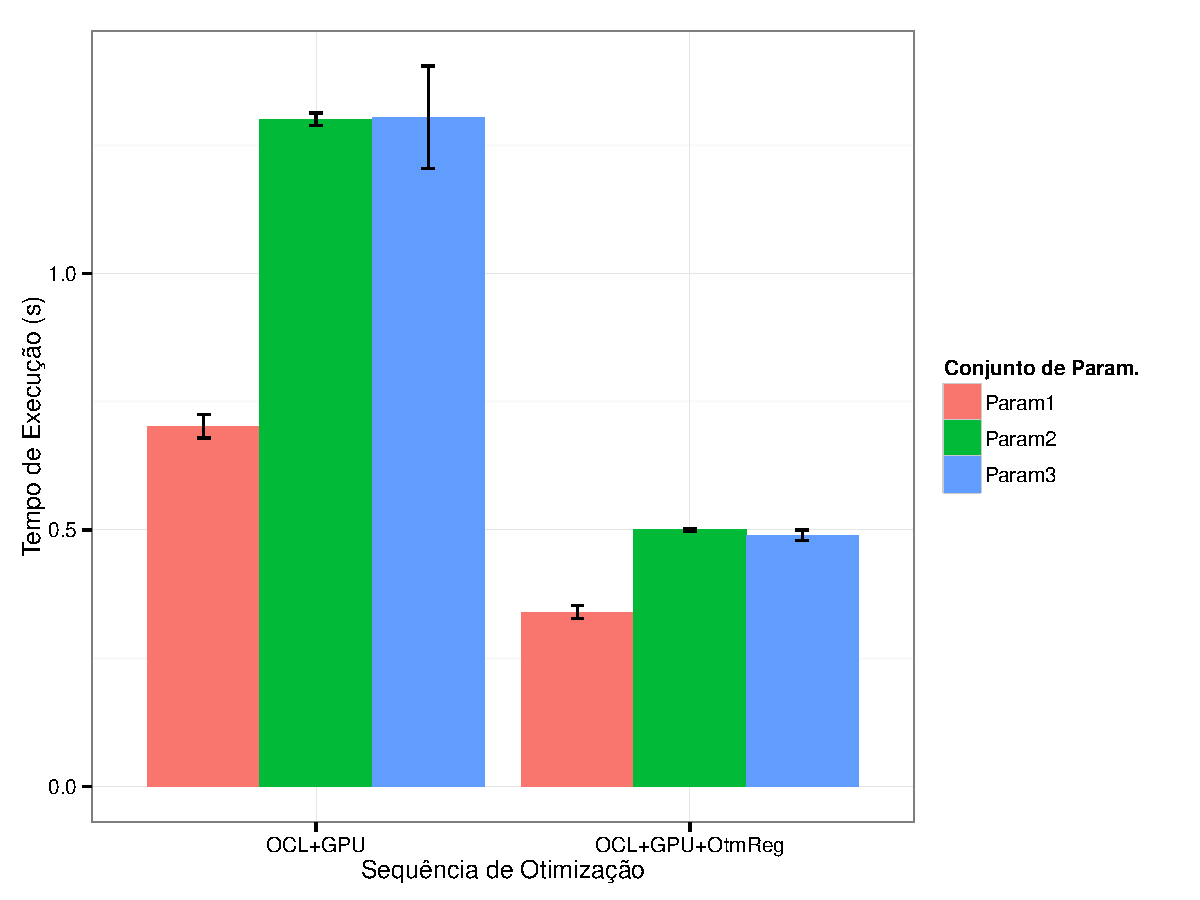
\includegraphics[width=0.8\textwidth]{oclpressure.pdf}
\caption{Tempos de execução do código com OpenCL com \textit{inlining} sobre a GPU antes e depois de mover os dados para memória de constantes.}
\label{fgclpressure}
\end{figure}

\subsection{Otimizações Não Implementadas ou Não Mantidas}

Falar sobre o fato que algumas otimizações não foram aplicadas.

\subsubsection{Vetorização}

Falar sobre vetorização no OpenCL e como tentamos aplicar, mas que não houve nenhum benefício.

\subsubsection{\textit{Loop Blocking}}

Argumentar que o código não é memory bound e que blocking não seria eficiente.

\section{Trabalhos Futuros}

Falar sobre analisar o código sobre uma ferramenta sofisticada e investigar se estamos próximos do limite teórico do hardware.

Falar sobre aplicar essas otimizações sobre o OpenMP e medir o desempenho.

Falar sobre as posiveis otimizações que ainda podem ser aplicadas.

\section{Conclusão}

\begin{figure}[H]
\centering
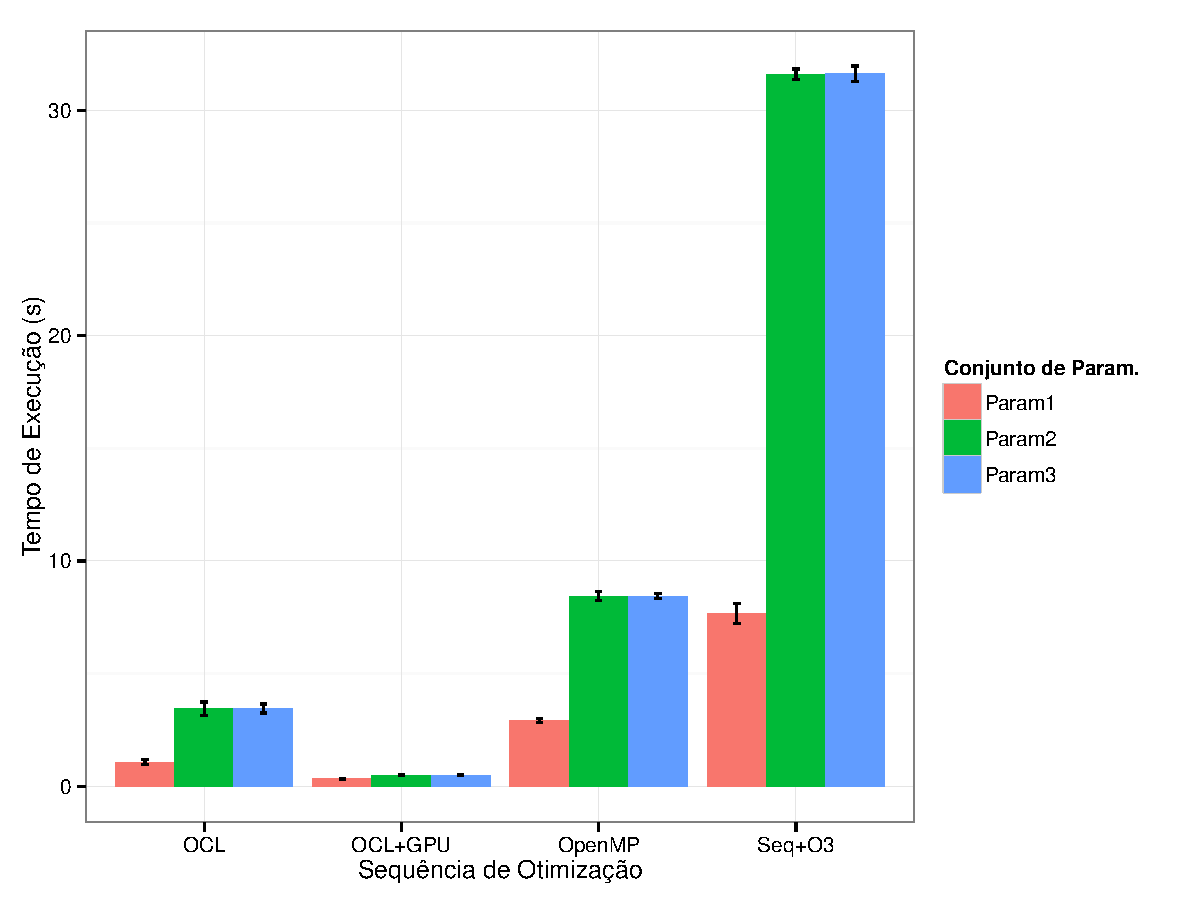
\includegraphics[width=0.8\textwidth]{final.pdf}
\caption{Tempos de execução do código com OpenCL com \textit{inlining} sobre a GPU antes e depois de mover os dados para memória de constantes.}
\label{fgclpressure}
\end{figure}

\begin{figure}[H]
\centering
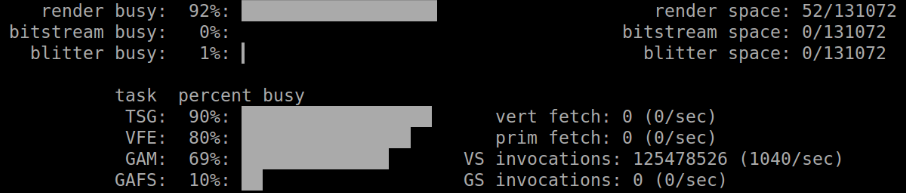
\includegraphics[width=0.8\textwidth]{ss.png}
\caption{Taxa de utilização da GPU durante a execução dos experimentos segundo o intel\_gpu\_top.}
\label{fss}
\end{figure}

Tentar analisar o desempenho teórico do hardware. Tentar argumentar o desempenho alcançado.

Falar sobre o OpenCL e as otimizações encontradas. Falar sobre os problemas e os trabalhos futuros.


\end{document}
